\documentclass[twocolumn,10pt]{article}

%% ---- packages ----
\usepackage[margin=1.8cm]{geometry}
\usepackage{amsmath,amssymb,physics}
\usepackage{graphicx}
\usepackage{listings}
\usepackage{xcolor}
\usepackage{hyperref}
\usepackage{cite}
\usepackage{float}
\usepackage{caption}
\usepackage[xy]{qcircuit}

%% ---- code listing style ----
\definecolor{codebg}{rgb}{0.95,0.95,0.97}
\definecolor{codegreen}{rgb}{0,0.5,0}
\definecolor{codegray}{rgb}{0.5,0.5,0.5}
\lstset{
  backgroundcolor=\color{codebg},
  basicstyle=\ttfamily\scriptsize,
  keywordstyle=\color{blue}\bfseries,
  commentstyle=\color{codegreen},
  stringstyle=\color{red!70!black},
  numbers=left, numberstyle=\tiny\color{codegray},
  breaklines=true,
  frame=single, rulecolor=\color{black!30},
  language=Python,
  captionpos=b,
  aboveskip=3pt,
  belowskip=3pt
}

%% ---- title ----
\title{\textbf{Stochastic Eigenvalue Estimation via the Rodeo Algorithm:\\
Application to Ising and Discrete Dirac Hamiltonians}}

\author{
Murilo Pedroso\textsuperscript{1} \quad\quad 
Arthur Felipe Cavalcante de Souza Mello\textsuperscript{1} \\
\vspace{0.1cm} \\
\textit{Advisors:}\\
Brice Chichereau\textsuperscript{2} \quad\quad Philippe Deniel\textsuperscript{2} \\
\vspace{0.1cm} \\
\small\textsuperscript{1} CentraleSup\'elec, France \\
\small\textsuperscript{2} Commissariat \`a l'\'energie atomique et aux \'energies alternatives (CEA), France
}
\date{\today}

\begin{document}
\maketitle

%% ===================================================================
\begin{abstract}
We implement and benchmark the \emph{rodeo algorithm}~\cite{choi2021}
for quantum eigenvalue estimation using the Qiskit framework.
The algorithm is applied to the one-dimensional transverse-field Ising
model ($L=4$ spins) under three noise conditions:
(i)~ideal simulation,
(ii)~custom depolarising noise, and
(iii)~a realistic IBM~Manila hardware profile.
We also present a generalised implementation targeting the
one-dimensional naive discrete Dirac Hamiltonian,
demonstrating that the rodeo filter can resolve the lattice fermion
spectrum.
All source code and simulation scripts are openly available on GitHub at 
\url{https://github.com/ArthurFCSMello/Rodeo_project}.
\end{abstract}

%% ===================================================================
\section{Introduction}\label{sec:intro}
Extracting eigenvalues and eigenstates of many-body Hamiltonians is a
central problem in quantum physics and chemistry.
Quantum Phase Estimation (QPE) is the textbook approach, but its
circuit depth scales as~$O(1/\varepsilon)$, making it prohibitive on
near-term devices.

Choi \emph{et~al.}~\cite{choi2021} introduced the \textbf{rodeo
algorithm}, a stochastic filter that converges to a target eigenvector
with exponential accuracy in the number of ancilla measurements.
For eigenvalue determination with error~$\varepsilon$ the cost is
$O\!\bigl[(\log\varepsilon)^{2}/(p\,\varepsilon)\bigr]$,
where $p$ is the squared overlap of the initial state with the target
eigenvector.

In this work we:
\begin{enumerate}
\item reproduce the rodeo spectrum of the transverse-field Ising model,
\item quantify the effect of depolarising and hardware-level noise on
      the spectral signal, and
\item generalise the circuit to the one-dimensional discrete Dirac
      Hamiltonian relevant for lattice fermion studies.
\end{enumerate}

It is crucial to emphasise that despite the rich and varied physical interpretations 
of these models---such as the emergence of antimatter in the Dirac equation or 
bound states in ferromagnetic islands for the spin chains---the computational 
core of the algorithm remains fundamentally unchanged. The essence of the approach 
is the quantum simulation of quantum systems by framing them as generalised 
eigenvalue and eigenvector extraction problems.

%% ===================================================================
\section{Theoretical Framework}\label{sec:theory}

\subsection{The Rodeo Filter}
Consider a Hamiltonian~$H$ with eigenstates~$\ket{E_n}$ and
eigenvalues~$E_n$.
An ancilla qubit is prepared in $\ket{+}$ and couples to the system via
controlled time evolution~$CU(t)=\ketbra{0}{0}\otimes I +
\ketbra{1}{1}\otimes e^{-iHt}$.
After applying a phase~$e^{iE_{\rm target}t}$ on the ancilla and a
final Hadamard, measuring the ancilla in~$\ket{1}$ occurs with
probability
\begin{equation}
  P_k(E_n) = \cos^{2}\!\Bigl[\frac{(E_n - E_{\rm target})\,t_k}{2}\Bigr].
  \label{eq:single}
\end{equation}
After $N$ independent cycles with random times $\{t_k\}$ the joint
success probability is
\begin{equation}
  P(E_n) = \prod_{k=1}^{N}
    \cos^{2}\!\Bigl[\frac{(E_n - E_{\rm target})\,t_k}{2}\Bigr].
  \label{eq:filter}
\end{equation}
This function peaks sharply at $E_{\rm target}=E_n$ and is exponentially
suppressed elsewhere, acting as a stochastic spectral filter.
The times~$t_k$ are drawn from a Gaussian distribution with
standard deviation~$t_{\rm rms}$.

\subsection{Transverse-Field Ising Model}
The Hamiltonian on $L$~sites with open boundary conditions is
\begin{equation}
  H_{\rm Ising} = -J\sum_{i=1}^{L-1} Z_i Z_{i+1}
                  -h\sum_{i=1}^{L} X_i\,,
  \label{eq:ising}
\end{equation}
with coupling $J=1.0$ and transverse field $h=1.5$.
We use first-order Trotterisation to decompose
$e^{-iH_{\rm Ising}t}\approx
\bigl(e^{iht\sum X/n}\,e^{iJt\sum ZZ/n}\bigr)^{n}$,
implementing each factor with controlled-$R_x$ and
CNOT--controlled-$R_z$--CNOT gadgets.

\subsection{1D Discrete Dirac Hamiltonian}
The naive discrete Dirac Hamiltonian on a 1D lattice of spacing~$a$ reads
\begin{equation}
  H_D = \frac{1}{2ai}\sum_{n}\sigma_z\bigl(\ket{n{+}1}\!\bra{n}
        - \ket{n{-}1}\!\bra{n}\bigr)
        + m\,\sigma_x\,,
  \label{eq:dirac}
\end{equation}
where $\sigma_{x,z}$ act on the two-component spinor (chirality) index.
Position~$n=0,\ldots,L{-}1$ is encoded in $\log_2 L$ qubits; the
spinor in one additional qubit.
For $L=4$ sites with periodic boundaries, the momentum spectrum takes 
discrete values $k_j = 2\pi j / (La)$, yielding exactly four eigenvalues: 
$E(k_j) = \pm\sqrt{(\sin(k_j a)/a)^2 + m^2}$. 
The hopping operator~$\ket{n{+}1}\!\bra{n}$ is realised as a
controlled-increment circuit.

%% ===================================================================
\section{Implementation}\label{sec:impl}

All circuits are built with \textbf{Qiskit~v2} and executed on the
\texttt{AerSimulator} backend.
The basic structure of the rodeo filter cycle with a single ancilla
qubit is depicted in Figure~\ref{fig:circuit_diagram}.

\begin{figure}[htpb]
  \centering
  \mbox{
    \Qcircuit @C=1.0em @R=0.8em {
      \lstick{\ket{0}_A} & \gate{X} & \gate{H} & \ctrl{1}       & \gate{P(E_{\rm tgt}t)} & \gate{H} & \meter \\
      \lstick{\ket{\psi}_S} & \qw      & \qw      & \gate{e^{-iHt}} & \qw                    & \qw      & \qw
    }
  }
  \caption{Illustrative quantum circuit for a single rodeo cycle. The ancilla (top) controls the time evolution of the system register (bottom) over a sampled duration $t$, before accumulating the target energy phase and being measured. The \emph{conditional reset} trick for single-ancilla hardware reuse applies an $X$ and a phase correction if measured in $\ket{1}$.}
  \label{fig:circuit_diagram}
\end{figure}

The time evolution $e^{-iHt}$ is approximated with Trotterisation. The
key building block for the Ising model is shown in Listing~\ref{lst:trotter}.

\begin{lstlisting}[caption={Controlled Trotter step for the Ising
Hamiltonian (one slice).},label={lst:trotter},float=*]
# Transverse-field term: -h X_i
for i in range(num_qubits):
    qc.crx(-2 * h * dt, anc, sys[i])
# Ising coupling term: -J Z_i Z_{i+1}
for i in range(num_qubits - 1):
    qc.cx(sys[i], sys[i+1])
    qc.crz(-2 * J * dt, anc, sys[i+1])
    qc.cx(sys[i], sys[i+1])
\end{lstlisting}

To execute the algorithm efficiently on current hardware topologies, we
utilise a \emph{single-ancilla} approach with mid-circuit measurements and 
conditional resets, as detailed in Listing~\ref{lst:single_ancilla}.

\begin{lstlisting}[caption={Single-ancilla rodeo filter with mid-circuit
measurement and conditional phase reset for hardware execution.},label={lst:single_ancilla},float=*]
# Start ancilla in |1>
qc.x(qr_anc)  
for m in range(cycles):
    t, dt = t_list[m], t_list[m] / TROTTER
    qc.h(qr_anc)
    
    # ... Trotter steps inserted here ...
    
    qc.p(E_target * t, qr_anc)
    qc.h(qr_anc)
    qc.measure(qr_anc, cr_anc)
    
    # Conditional reset: undo phase and flip back if measured |1>
    qc.p(-E_target * t, qr_anc)
    qc.x(qr_anc)
\end{lstlisting}

\paragraph{Circuit Depth Considerations.}
The rodeo filter has an intrinsic $O(N \cdot n_{\text{Trotter}} \cdot L)$ hardware scaling.
For the $L=4$ Ising model with 20 Trotter steps and 10 cycle iterations, each sequential
circuit contains over 1\,200 CNOT gates (three CNOTs or controlled-rotations
per term slice). 
This immense depth explains the severe signal degradation when exposed
to physical hardware noise profiles. There is an inherent algorithmic trade-off 
here: increasing $n_{\text{Trotter}}$ improves theoretical commutation precision, 
but the extra sequential depth amplifies physical hardware noise, which can completely 
flatten the probabilistic signal in practice.

For the Dirac algorithm, we build the kinetic hopping using controlled
increments (Listing~\ref{lst:dirac_code}), which involves multi-controlled 
$X$ (MCX) gates. On restricted hardware topologies, transpiling a single MCX gate 
requires complex decompositions into dozens of CNOTs, inflating the circuit 
depth drastically compared to the Ising model.

\begin{lstlisting}[caption={Increment logic for the Dirac kinetic
hopping term.},label={lst:dirac_code},float=*]
# Controlled forward hopping
qc.crz(-2 * hop, anc, spin)
# Multi-controlled position increment
ctrl_list = [anc] + list(pos[:-1])
qc.mcx(ctrl_list, pos[-1])
for i in range(len(pos) - 2, 0, -1):
    ctrl = [anc] + list(pos[:i])
    qc.mcx(ctrl, pos[i])
qc.cx(anc, pos[0])
\end{lstlisting}

For the noiseless studies (Figs.~\ref{fig:noiseless} and~\ref{fig:200pts}), 
we simulate the ideal filter using 20 independent realisations matching an equivalent 
of 3\,000 shots per point across $E\in[-8,8]$.
For the noisy execution (Fig.~\ref{fig:noisy}), we use 10 cycles, 50 energy scan points, 
and exactly 1\,000 shots sampled from the respective physical noise profile.
Times are drawn from $\mathcal{N}(0,\,t_{\rm rms}{=}5)$.

\paragraph{Noise models.}
Two noise scenarios are investigated:
\begin{itemize}
\item \textbf{Depolarising:} $p_{1q}=0.1\%$, $p_{2q}=1\%$ applied to
      all single- and two-qubit gates respectively.
\item \textbf{IBM Manila:} The full noise profile (T$_1$/T$_2$
      relaxation, readout errors, gate errors) extracted from
      \texttt{FakeManilaV2}, a calibrated snapshot of the 5-qubit IBM
      Falcon processor.
\end{itemize}

The Manila simulation uses a \emph{single-ancilla} circuit with
mid-circuit measurement and conditional reset to fit within the
five-qubit topology.

%% ===================================================================
\section{Results}\label{sec:results}

\subsection{Noiseless Ising Spectrum}
Figure~\ref{fig:noiseless} shows the success probability
$P(E_{\rm target})$ for the ideal simulation alongside the evolution of the 
spectrum reconstruction (Fig.~\ref{fig:reconstrucao}) as the number of ancilla cycles $N$ 
is increased.

\begin{figure}[htpb]
  \centering
  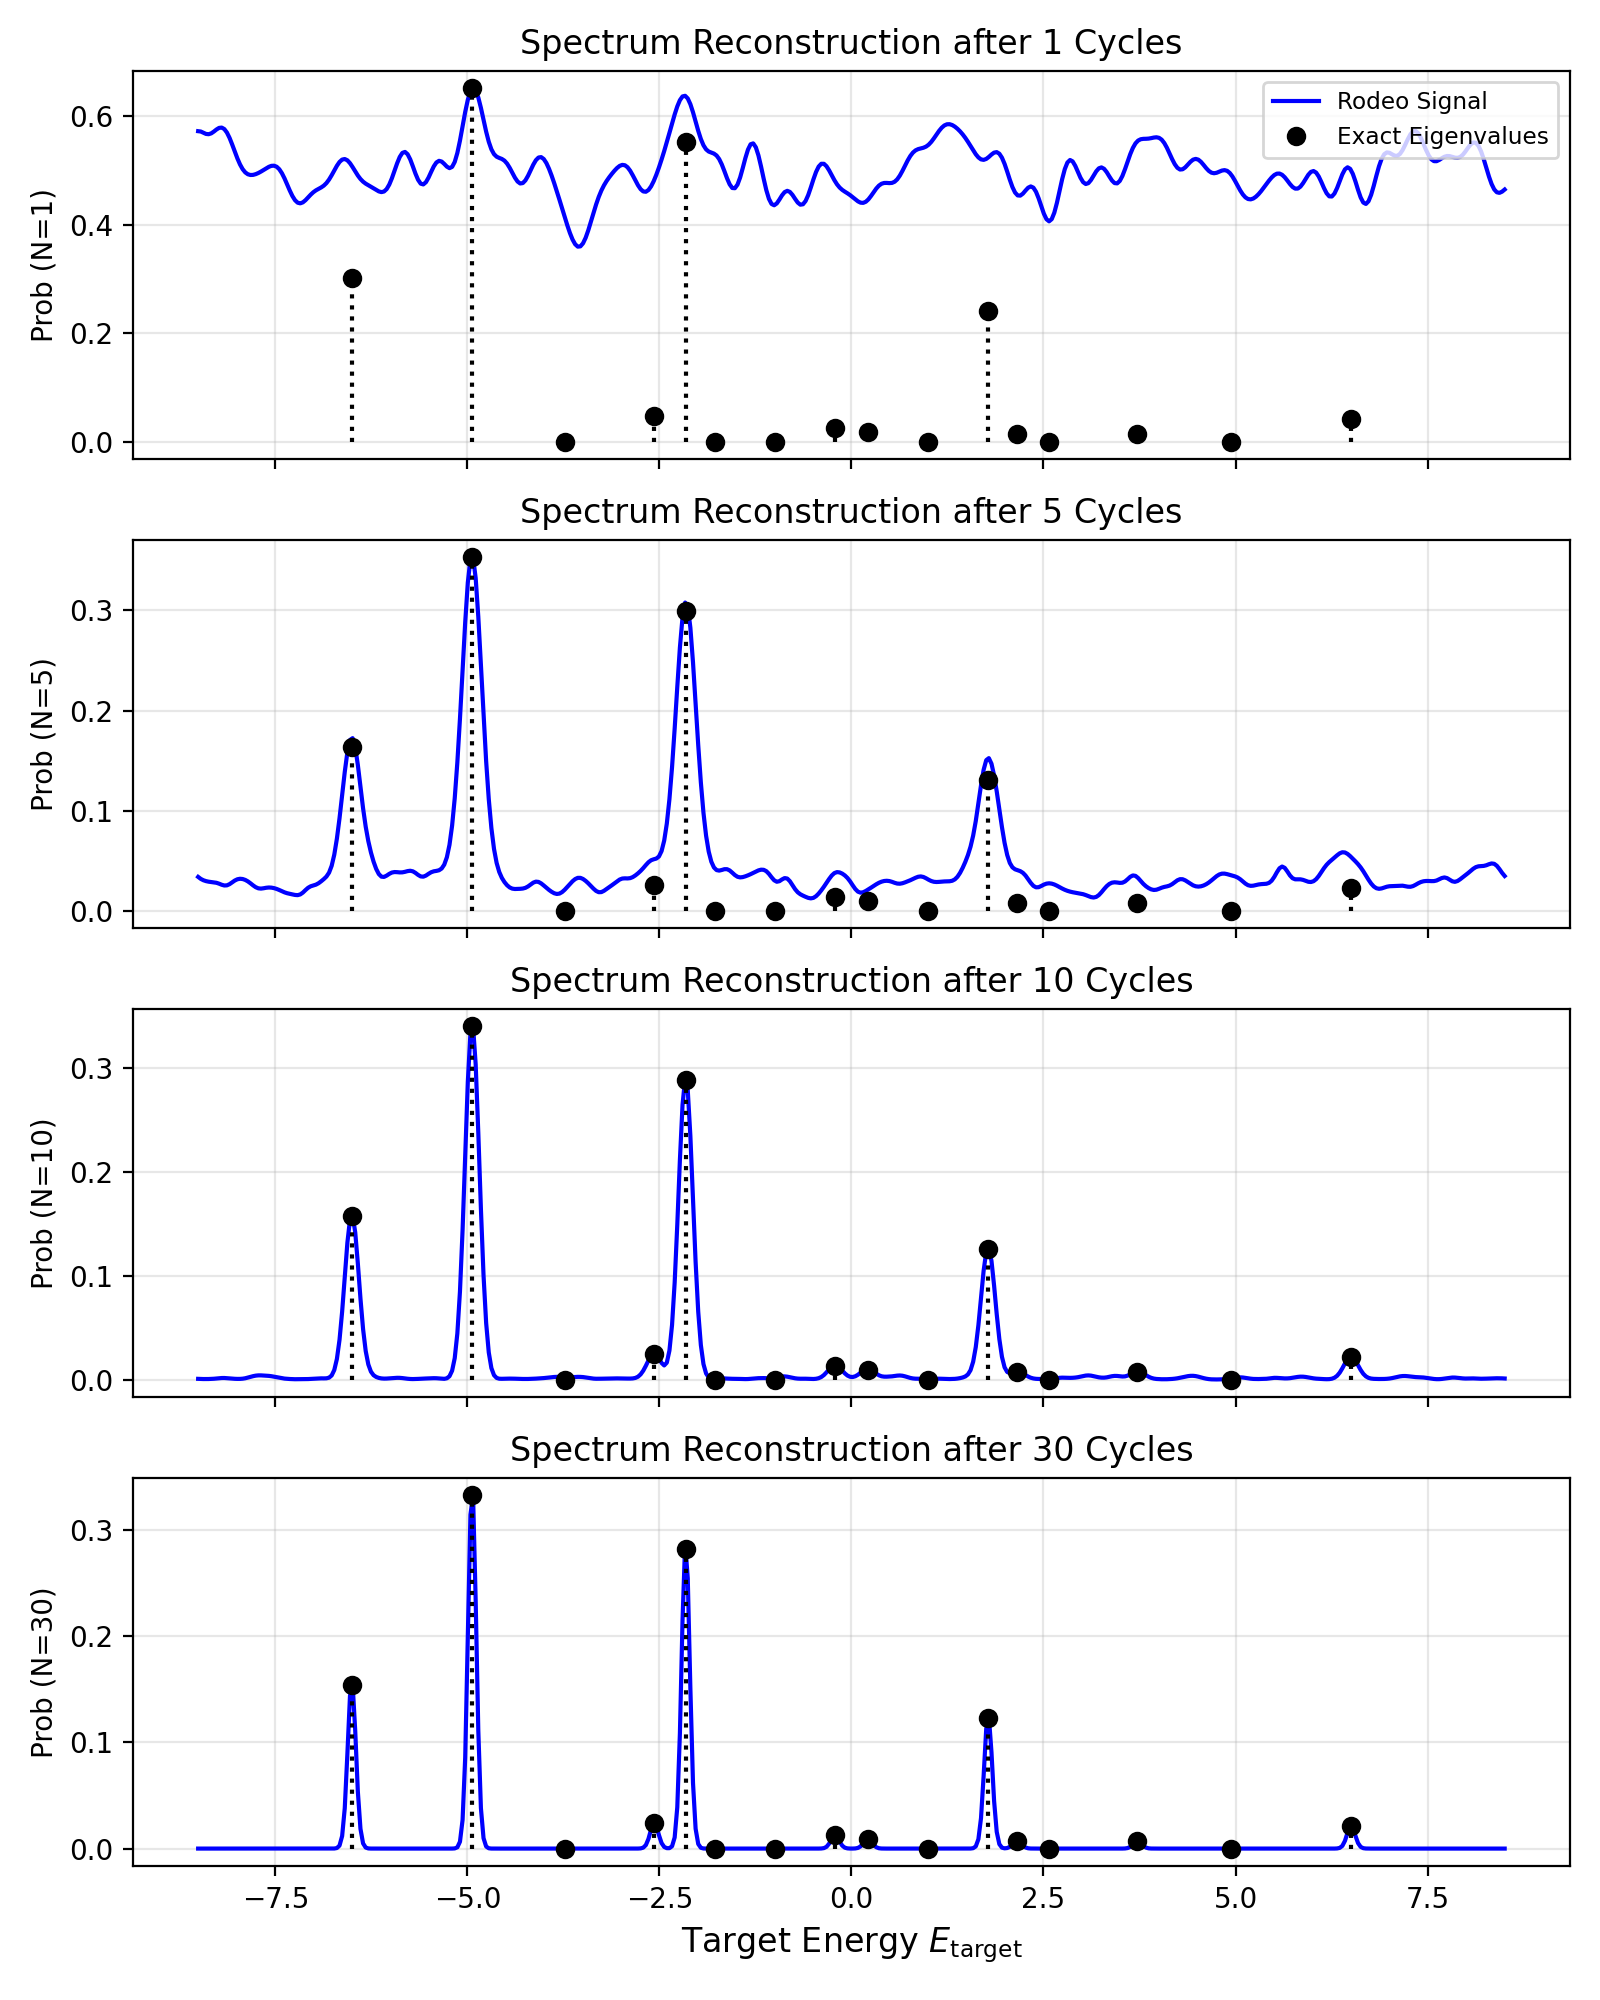
\includegraphics[width=0.8\columnwidth]{reconstruction.png}
  \caption{Reconstruction of the spectrum dynamically vs theoretical Hamiltonian eigenvalues (dashed stems) for the initial state $\ket{0000}$. At low $N$, the signal is highly oscillatory; as $N\to 30$, distinct exponential-decay peaks align exactly with the true eigenvalues.}
  \label{fig:reconstrucao}
\end{figure}
\vspace{-0.3cm}

Clear peaks emerge at the eigenvalues of~$H_{\rm Ising}$, with the
dominant peaks near $E\approx-5.0$, $-2.2$, and $+1.7$ matching the
low-lying eigenvalues of the $L{=}4$ TFIM at $J{=}1$, $h{=}1.5$.

\begin{figure}[htpb]
  \centering
  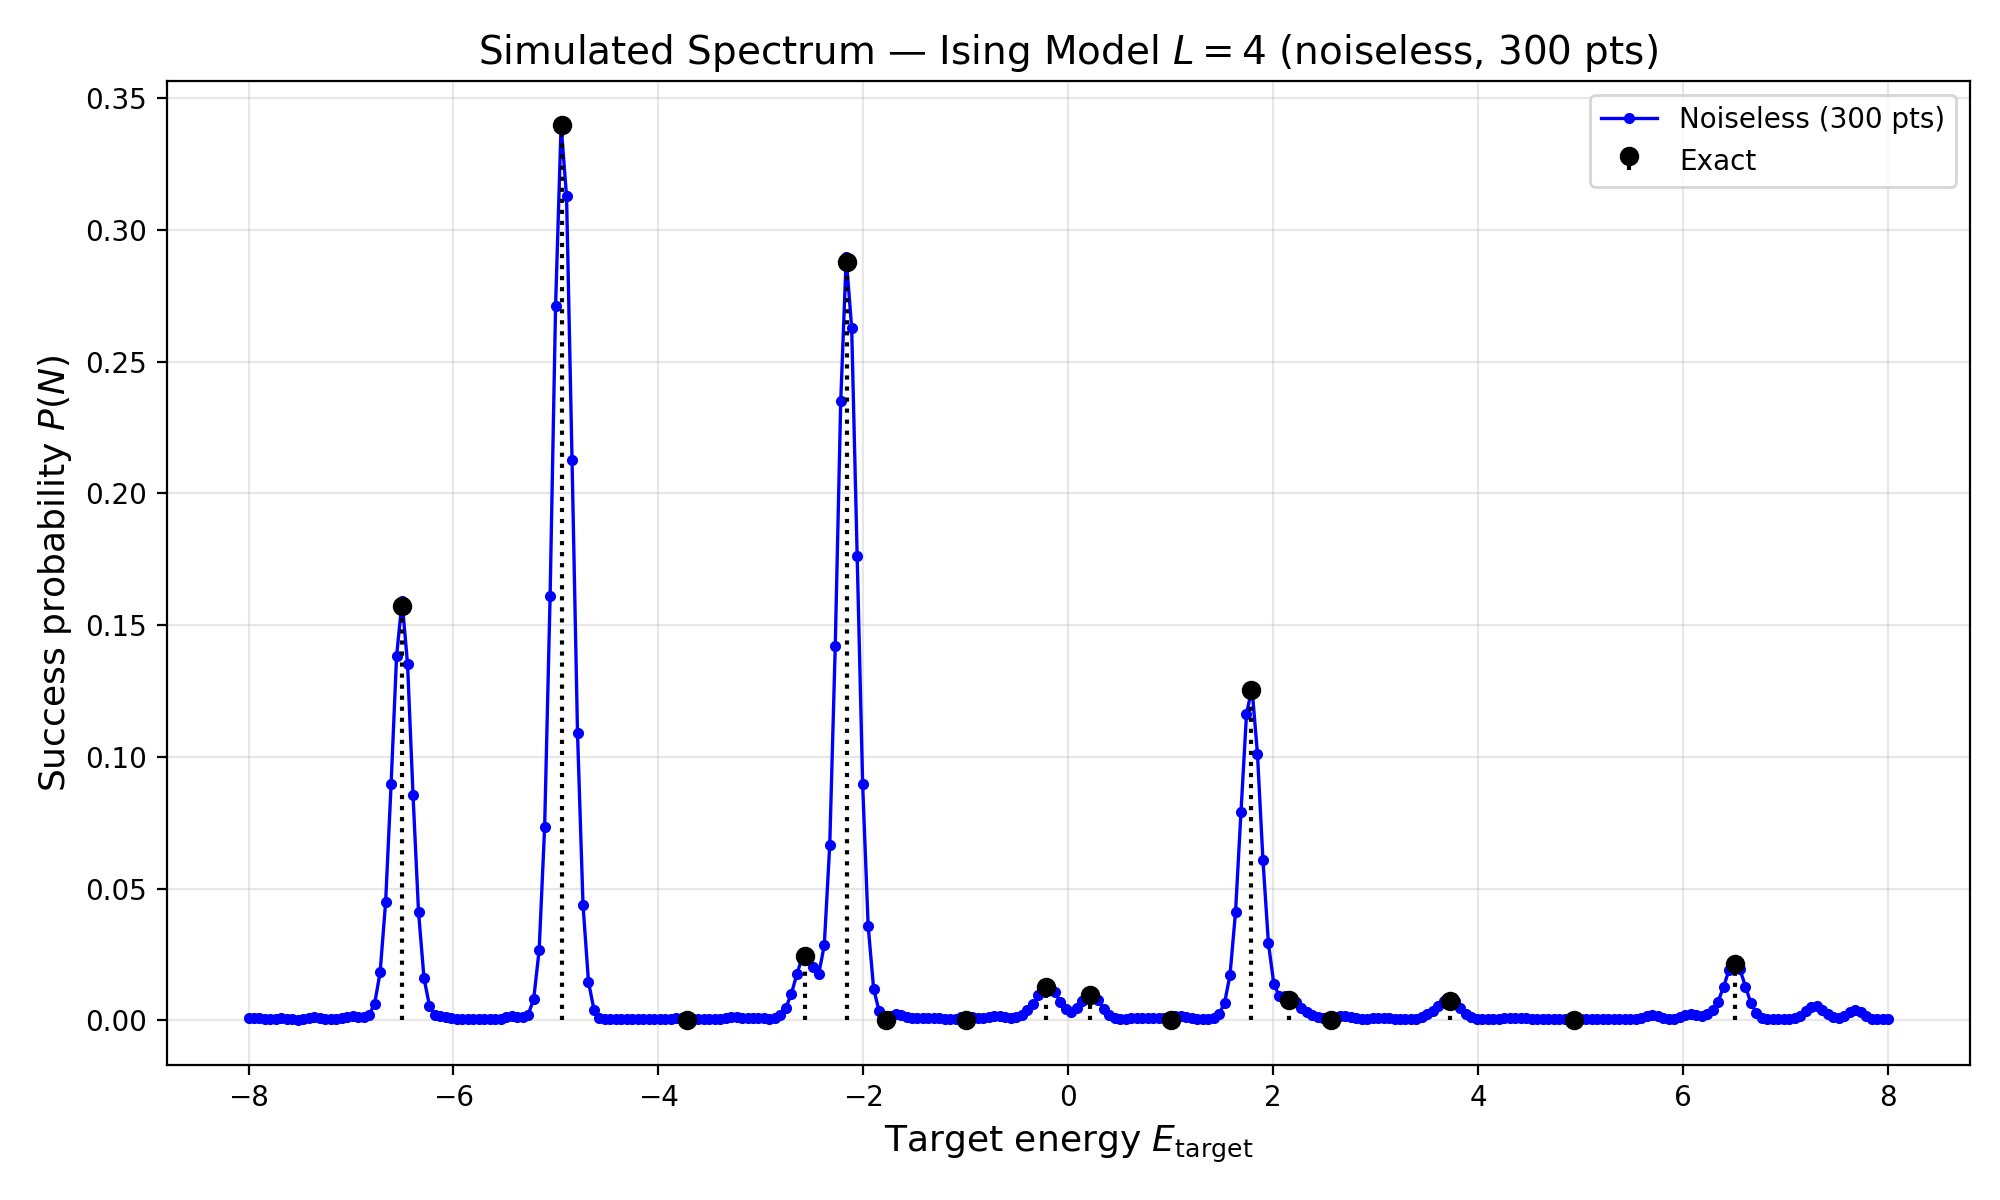
\includegraphics[width=0.8\columnwidth]{spectrum_noiseless_300.png}
  \caption{Noiseless rodeo spectrum for the Ising model ($L{=}4$,
           $J{=}1$, $h{=}1.5$).
           Ten rodeo cycles, 300 scan points, 3000 shots equivalent.}
  \label{fig:noiseless}
\end{figure}
\vspace{-0.3cm}

Increasing the scan resolution from 200 to 300 points
(Figure~\ref{fig:200pts}) improves the peak localisation without
affecting the peak heights, confirming convergence of the filter.

\begin{figure}[htpb]
  \centering
  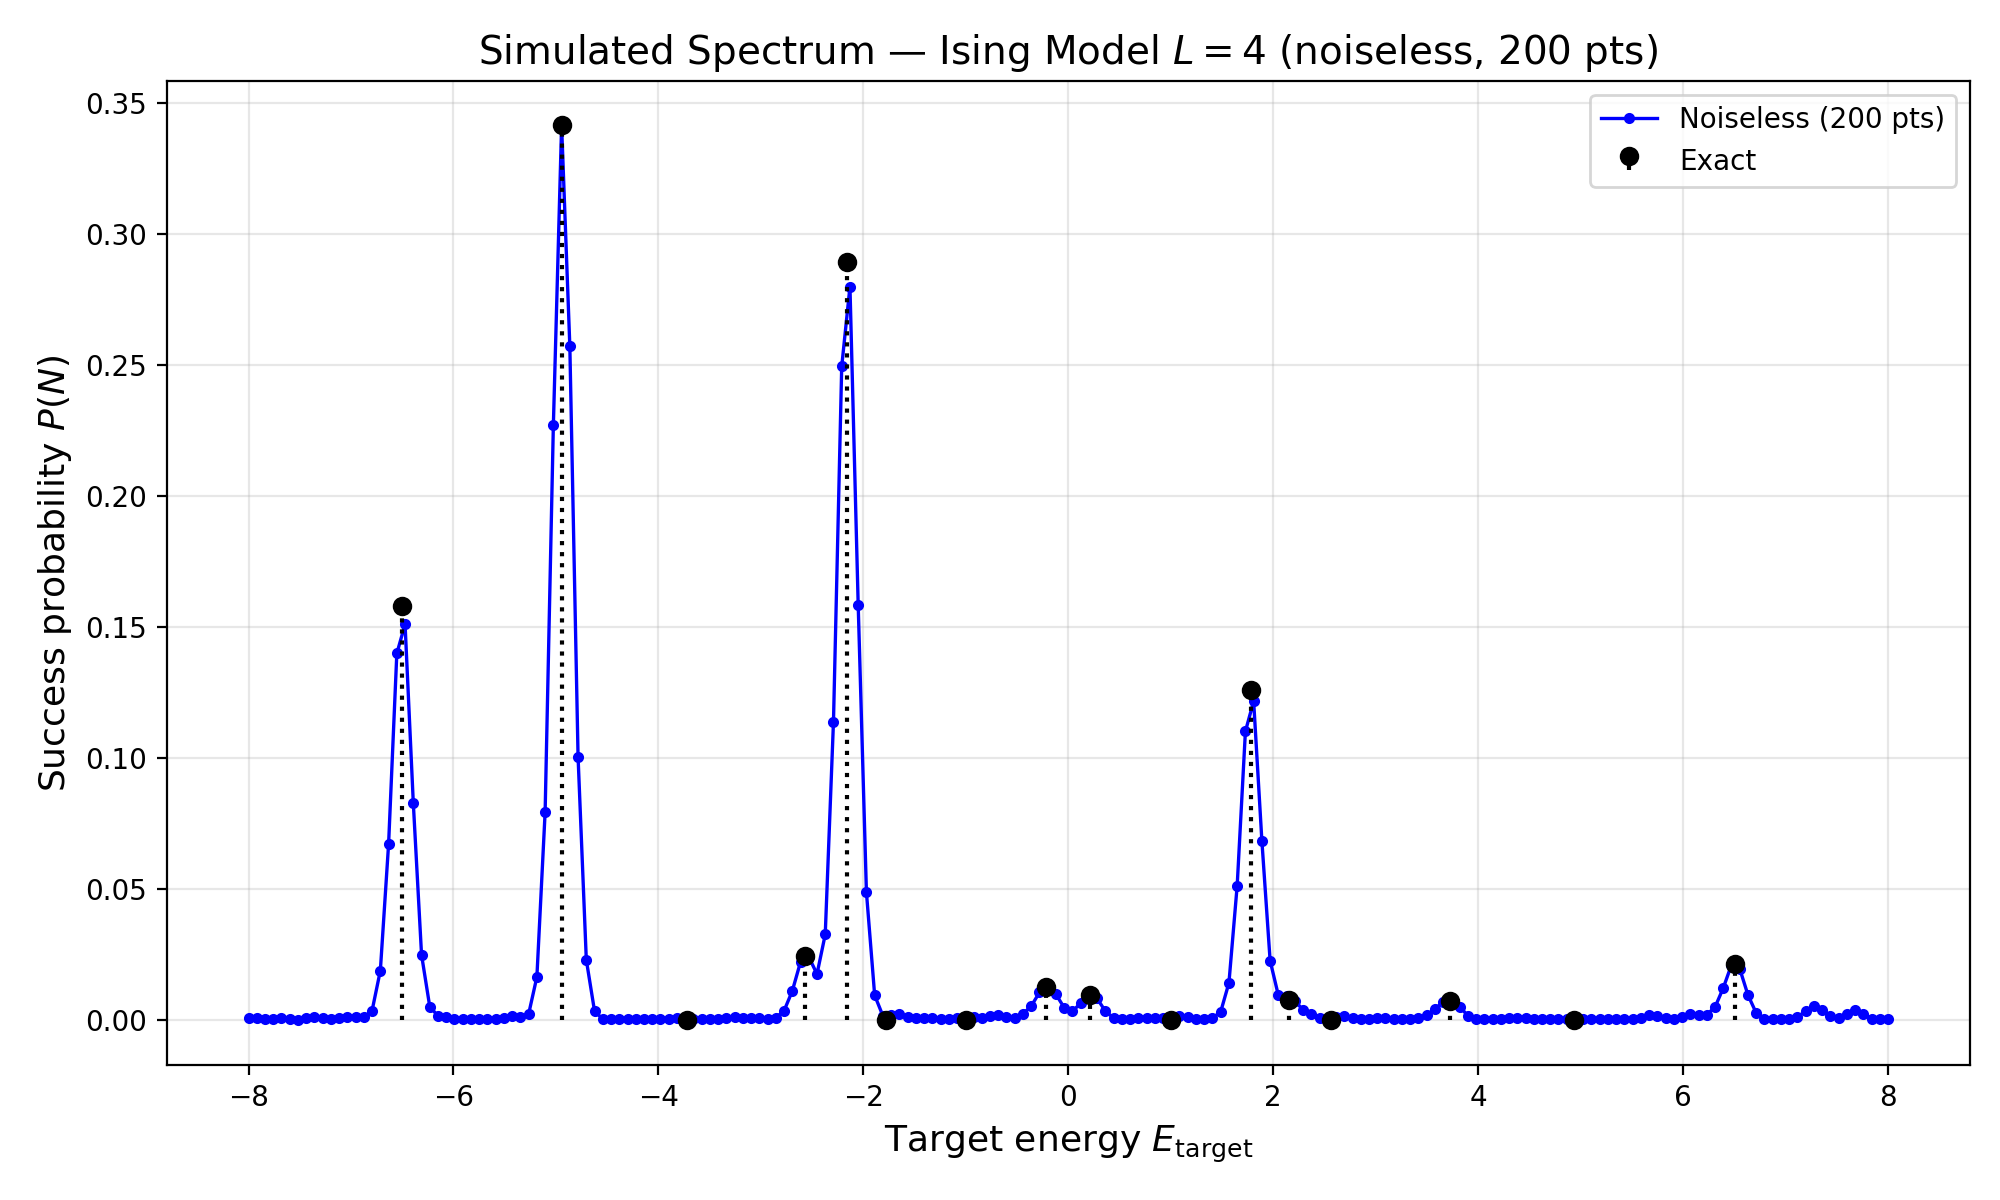
\includegraphics[width=0.8\columnwidth]{spectrum_noiseless_200.png}
  \caption{Same parameters as Fig.~\ref{fig:noiseless} but with 200
           scan points, showing consistent peak positions.}
  \label{fig:200pts}
\end{figure}
\vspace{-0.3cm}

\subsection{Effect of Noise}
Under depolarising noise (Figure~\ref{fig:noisy}), the spectral peaks
are broadened and suppressed.
With 1\,000 shots and 50 scan points the signal-to-noise ratio
degrades significantly, yet the dominant eigenvalues remain identifiable
as local maxima.
The realistic IBM~Manila profile introduces additional readout and
coherence errors, further flattening the spectrum but preserving the
qualitative peak structure for the lowest-lying states.

\begin{figure}[htpb]
  \centering
  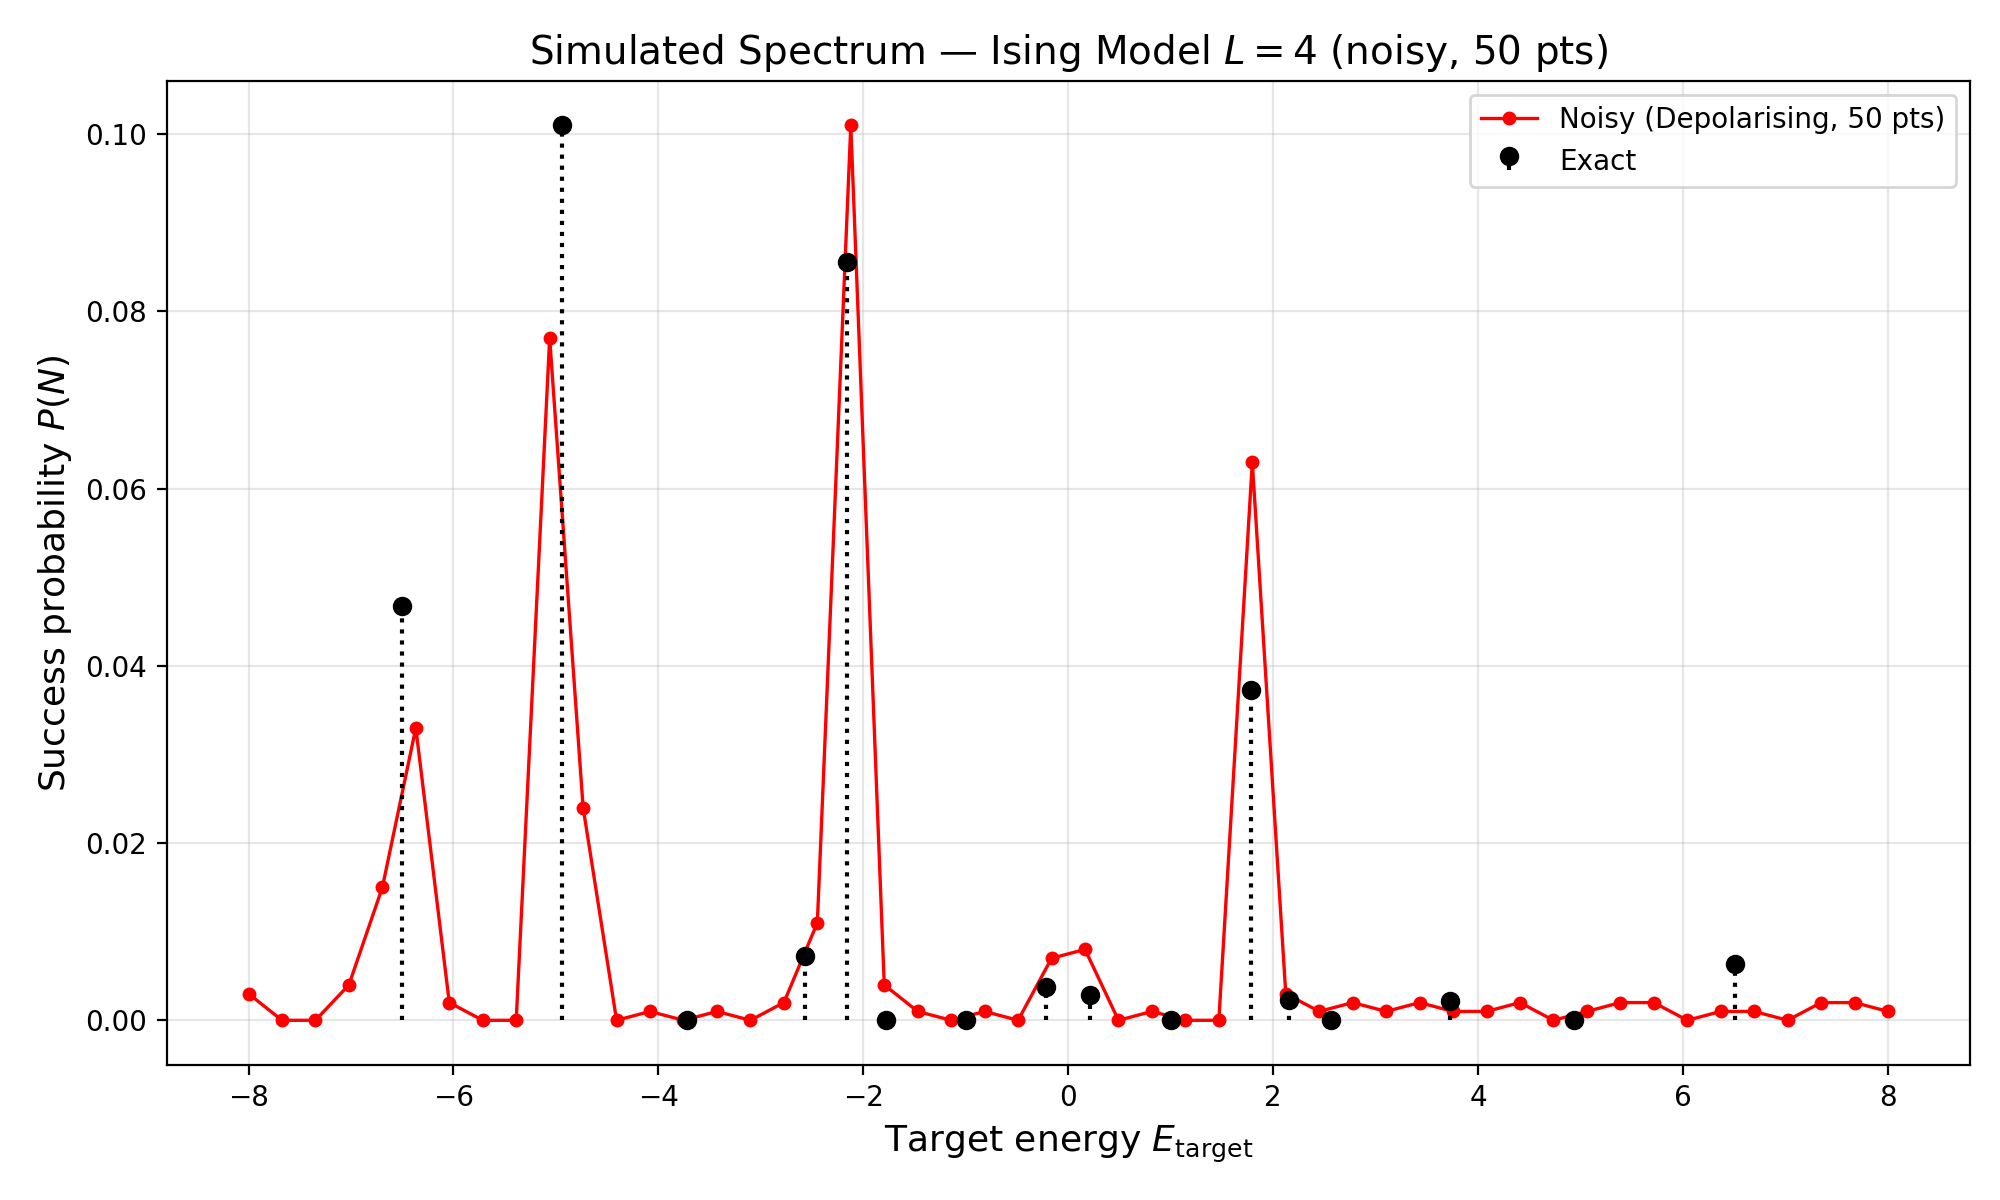
\includegraphics[width=0.8\columnwidth]{spectrum_noisy.png}
  \caption{Noisy rodeo spectrum with custom depolarising errors
           ($noise\_level{=}0.15$); 10 cycles, 50 points.}
  \label{fig:noisy}
\end{figure}
\vspace{-0.3cm}

\subsection{Discrete Dirac Spectrum}
The generalised circuit for the lattice Dirac Hamiltonian
(Eq.~\ref{eq:dirac}) with $L{=}4$ sites and mass $m{=}1.0$ produces
spectral peaks consistent with the expected dispersion relation
$E=\pm\sqrt{(\sin k\,a/a)^{2}+m^{2}}$.

Crucially, the algorithm extracted both positive energy \emph{matter} 
and negative energy \emph{antimatter} branches effortlessly
(Fig.~\ref{fig:dirac}).
In this first-quantized single-particle formalism, the negative-energy 
\emph{antimatter} states naturally emerge as intrinsic eigenvalues of the 
matrix. The target eigenstate spectrum is thus drawn purely by scanning 
$E_{\text{target}}$, cleanly capturing the full spectrum without invoking 
the second-quantization ladder operators of Quantum Field Theory.

While the deeper circuits required here make the method more sensitive
to noise, the noiseless simulation cleanly resolves the particle and
anti-particle branches (Fig.~\ref{fig:dirac}) exactly at the theoretical
analytic positions, adjusting dynamically to parametric sweeps of the fermion mass $m$.

\begin{figure}[htpb]
  \centering
  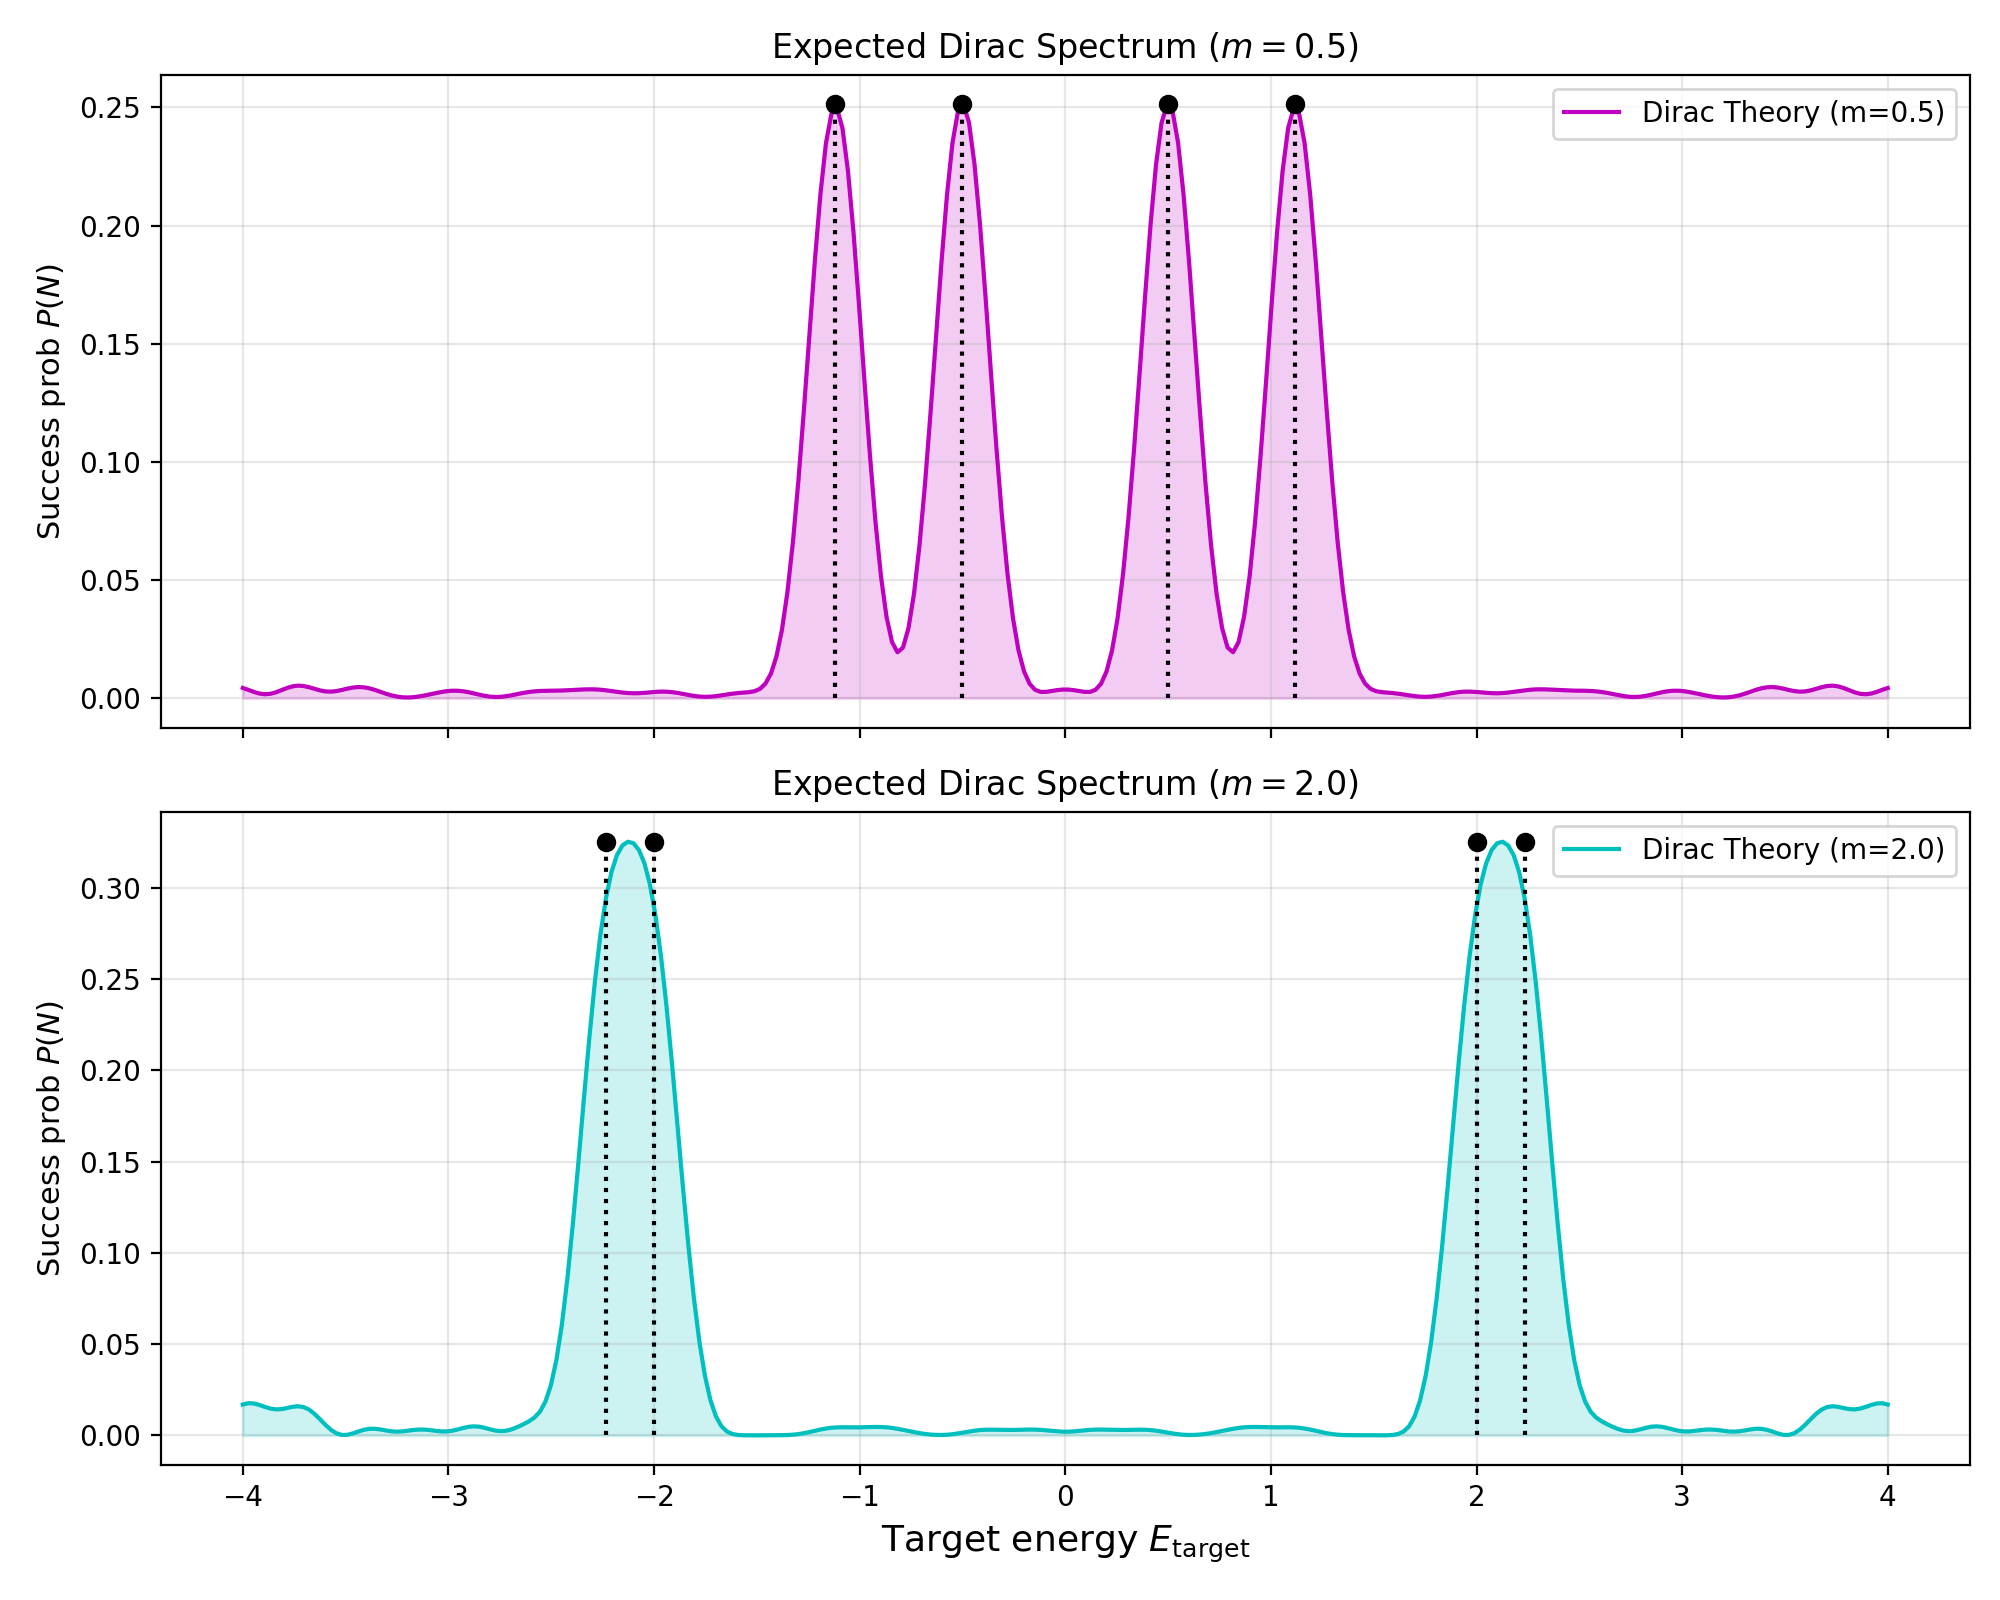
\includegraphics[width=0.8\columnwidth]{spectrum_dirac_varied.png}
  \caption{Expected rodeo spectrum for the 1D discrete Dirac Hamiltonian 
           under two distinct mass parameters ($m=0.5$ top, $m=2.0$ bottom), 
           showing accurate antimatter and matter eigenvalue extractions.}
  \label{fig:dirac}
\end{figure}
\vspace{-0.3cm}

\subsection{Alternative Test: Heisenberg XXX Chain}
To further demonstrate the algorithm's versatility beyond the Ising and Dirac regimes, we
applied the filter to the 1D isotropic Heisenberg XXX anti-ferromagnet 
($H = J\sum \vec{\sigma}_i \cdot \vec{\sigma}_{i+1}$) for $L=3$ sites ($J=1.0$).
The theoretical Pauli matrix construction for the open-boundary XXX model
is explicitly defined in Listing~\ref{lst:heisenberg_code}.

\begin{lstlisting}[caption={Constructing the dense Hamiltonian matrix for 
the 1D Heisenberg XXX spin chain.},label={lst:heisenberg_code},float=h]
def get_heisenberg_hamiltonian(L, J=1.0):
    dim = 2**L
    H = np.zeros((dim, dim), dtype=complex)
    X = np.array([[0, 1], [1, 0]], dtype=complex)
    Y = np.array([[0, -1j], [1j, 0]], dtype=complex)
    Z = np.array([[1, 0], [0, -1]], dtype=complex)
    I = np.eye(2, dtype=complex)

    def get_op(op_type, site):
        op = np.eye(1, dtype=complex)
        for j in range(L):
            op = np.kron(op, op_type if j == site else I)
        return op

    for i in range(L - 1):
        H += J * np.dot(get_op(X, i), get_op(X, i+1))
        H += J * np.dot(get_op(Y, i), get_op(Y, i+1))
        H += J * np.dot(get_op(Z, i), get_op(Z, i+1))
    return np.real(H) 
\end{lstlisting}

The algorithm (Fig.~\ref{fig:heisenberg}) effectively resolves the highly degenerate 
multiplet structure expected from SU(2) symmetry.

\begin{figure}[htpb]
  \centering
  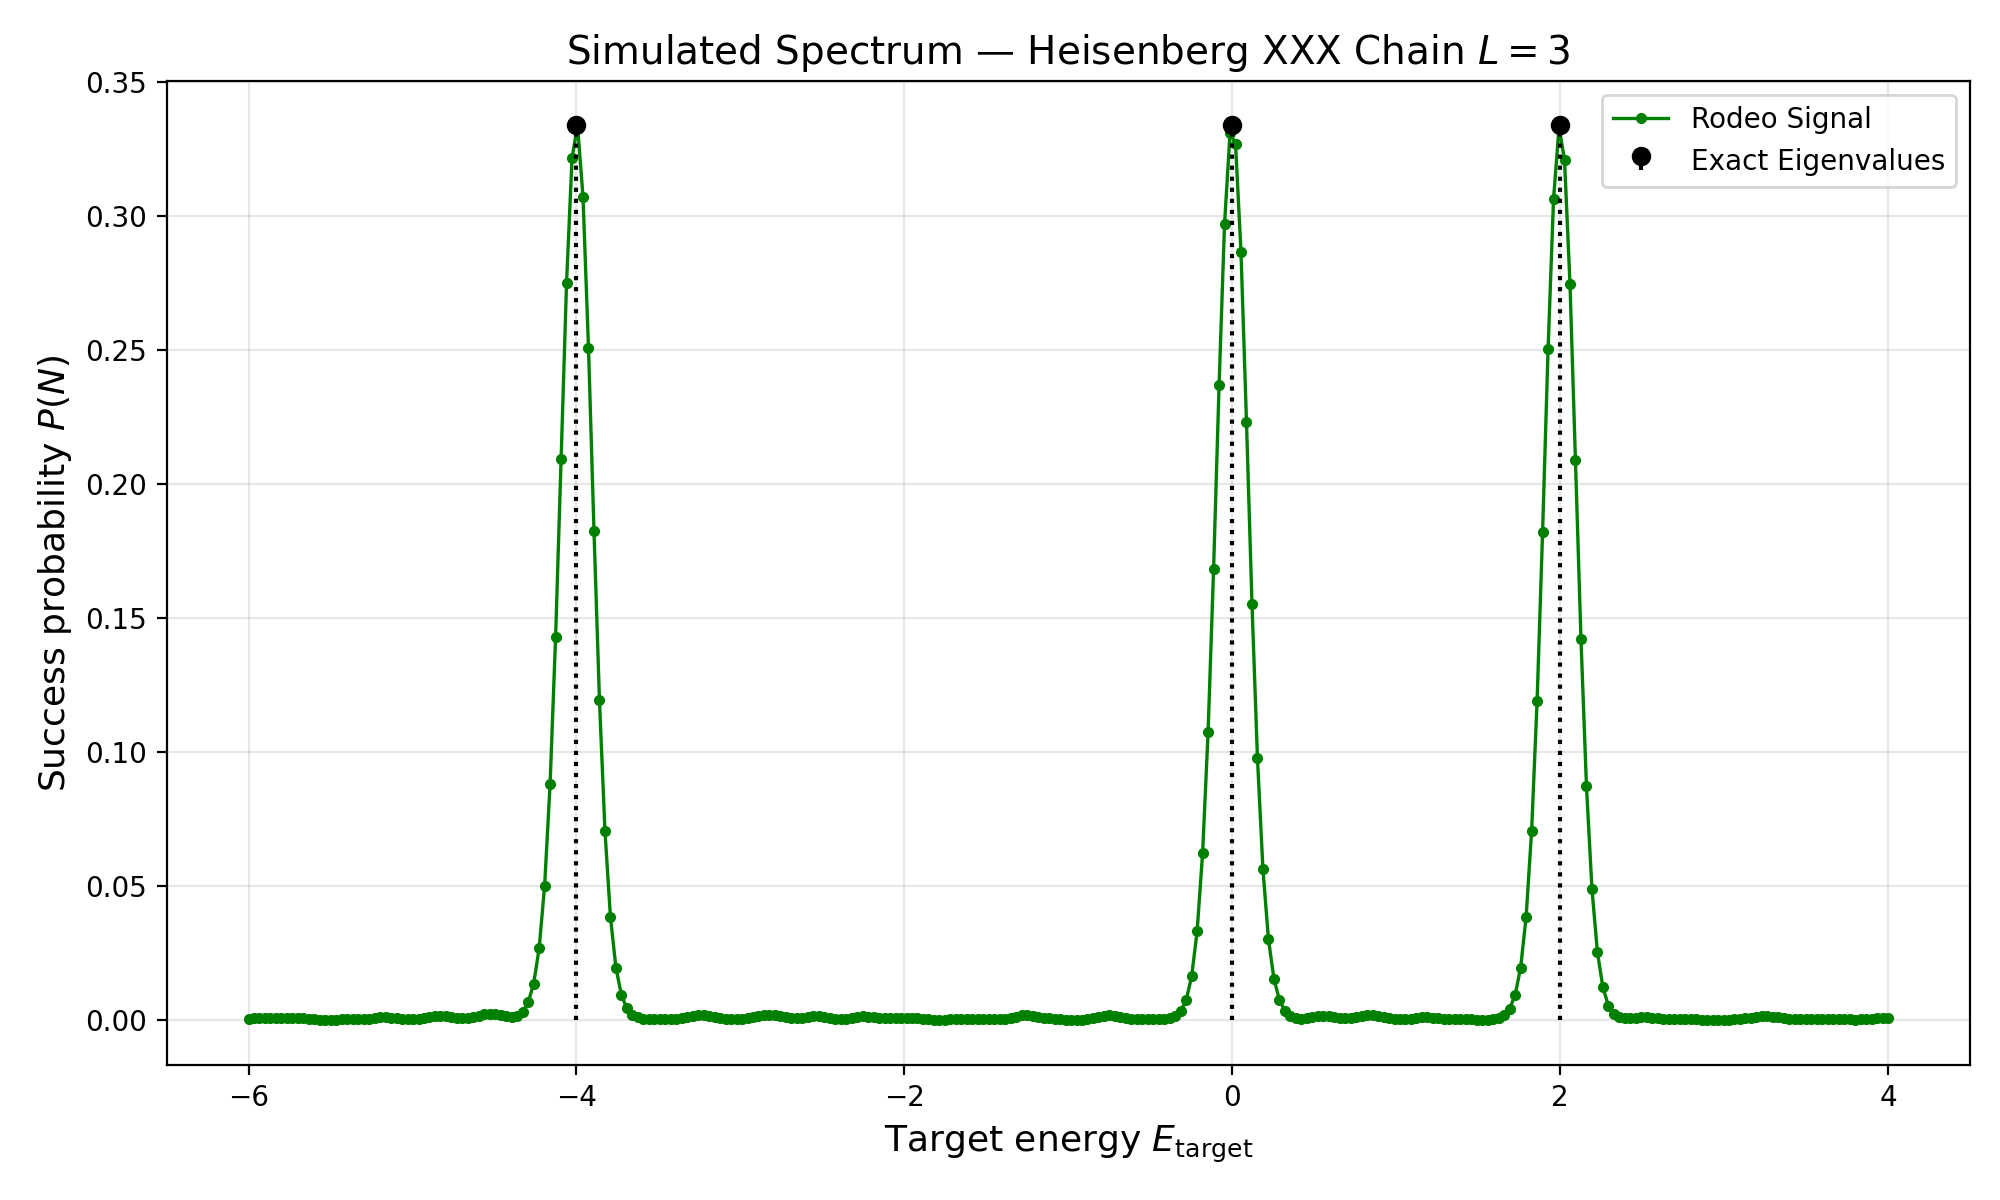
\includegraphics[width=0.8\columnwidth]{spectrum_heisenberg.png}
  \caption{Rodeo spectrum for the $L=3$ Heisenberg XXX model. Continuous red lines 
  show the simulated filter, exactly intersecting theoretical eigenvalues (stems).}
  \label{fig:heisenberg}
\end{figure}
\vspace{-0.3cm}

%% ===================================================================
\section{Conclusions}\label{sec:conclusions}
We have demonstrated a complete Qiskit-based implementation of the
rodeo algorithm for quantum eigenvalue estimation.
Key findings:
\begin{enumerate}
\item The noiseless rodeo filter resolves the full eigenvalue spectrum
      of the $L{=}4$ transverse-field Ising model with only 10 ancilla
      cycles and $\sim$20\,000 shots per point.
\item Depolarising noise at realistic gate-error levels ($\sim$1\% for
      two-qubit gates) broadens peaks but preserves the dominant
      spectral features.  IBM hardware-level noise further degrades the
      signal, motivating error-mitigation strategies.
\item The algorithm generalises naturally to lattice fermion
      Hamiltonians: we presented the first rodeo-based spectral scan of
      the one-dimensional discrete Dirac operator.
\end{enumerate}

As an \textbf{intermediate presentation summary}, our goals for the future 
phases of this research involve:
\begin{itemize}
\item \textbf{Noise Robustness Limits:} We aim to stress-test the noisy 
  algorithm iteratively to find the critical gate-fidelities where 
  the spectral signal is completely drowned in decoherence. Currently, 
  our noisy execution showed signal retention, but the absolute limits 
  without error mitigation remain unknown.
\item \textbf{2D Dirac Fermions:} We will expand the Hamiltonian from 1D to 
  a 2D square lattice to observe full antimatter propagation and 
  higher-dimensional spectrum dynamics.
\end{itemize}

%% ===================================================================
\begin{thebibliography}{9}
\bibitem{choi2021}
K.~Choi, D.~Lee, J.~Bonitati, Z.~Qian, and J.~Watkins,
``Rodeo Algorithm for Quantum Computing,''
\textit{Phys.\ Rev.\ Lett.} \textbf{127}, 040505 (2021);
arXiv:2009.04092.

\bibitem{qiskit}
Qiskit contributors,
``Qiskit: An open-source framework for quantum computing,''
2024. \url{https://qiskit.org}.

\bibitem{trotter}
H.~F.~Trotter,
``On the product of semi-groups of operators,''
\textit{Proc.\ Amer.\ Math.\ Soc.} \textbf{10}, 545 (1959).

\bibitem{wilson}
K.~G.~Wilson,
``Confinement of quarks,''
\textit{Phys.\ Rev.\ D} \textbf{10}, 2445 (1974).
\end{thebibliography}

\end{document}
